%%%%%%%%%%%%%%%%%%%%%%%%%%%%%%%%%%%%%%%%%%%
%
% szablon pracy licencjackiej 
% korzystający ze stylu pracalicmgr.cls
% 2017.03.22 K. Turzynski
% 2017.03.01 P. Durka durka@fuw.edu.pl 
% na podstawie pliku J. Żygierewicz 2016
%
%%%%%%%%%%%%%%%%%%%%%%%%%%%%%%%%%%%%%%%%%%%

\documentclass{pracalicmgr}
\usepackage{array}
\usepackage{graphicx}
\usepackage{multirow}
%\usepackage[margin = 0.5in, top = 0in]{geometry}
\usepackage{hyperref}
\usepackage{amsmath}
\usepackage{url}
\usepackage{float}
\usepackage{physics}
\usepackage{natbib}
\usepackage[utf8x]{inputenc}
\usepackage[T1]{fontenc}
\usepackage[english]{babel}
\usepackage[nottoc]{tocbibind}
\usepackage{lipsum}  
\usepackage{courier}
\author{Mateusz Kapusta}


\nralbumu{431289}

\title{Search for dormant Black Holes in OGLE survey database.}

\tytulang{Poszukiwanie uśpionych czarnych dziur w bazach danych przeglądu OGLE.}

\kierunek{studiów fizyka}

%\specjalnosc{$<$Specjalność-o-ile-dotyczy$>$}

\opiekun{dr Przemysław Mróz \\Astronomical Observatory\\Warsaw University}

%\dziedzina{13.200}
%\dziedzina{13.2 Fizyka}

\date{NAN 2022 r.}

\keywords{Dormant Black Holes,}



\begin{document}
    \maketitle
    \let\cleardoublepage\clearpage
\begin{abstract}
    \lipsum[2,7]
\end{abstract}

\tableofcontents

\chapter{Introduction}
\hspace{1cm} According to current knowledge most of the massive stars end their evolution as black holes, further investigation suggest there exist $\mathcal{O}(10^8)$ 
stellar mass BH's \citep{brown_scenario_1994} in our galaxy. Despite huge theoretical expectations only few tens of such objects have been found up to day. Most of them either emit X-rays through
accretion mechanism or can distinguish themselves on dynamical ground. Search for X-ray emission nor exotic dynamical behaviour are viable method to search BH search.
In the first case binary system is typically composed of either low mass star which overflows it's Roche lobe
(BH-LMXB) or high mass star which is accreting mass onto companion BH via stellar wind. In first case X-ray emission mostly have transient character \citep{bambi_transient_2016}
making it hard to observe them due to the accretion disc instabilities \citep{lasota_disc_2001}. What is crucial to emphasize is relative small period of the Black Hole binaries 
which can be uncovered from X-ray emission as longest one reported today for confirmed BH binary is $33$ d (GRS1915+105), wider orbits decrease relative X-ray brightness decreasing
chances to detect such objects.
In recent years new stellar mass BH's candidates are being found due to the new methods based on the dynamical grounds. Noticeable cases include spectroscopic observations 
\citep{liu_wide_2019,jayasinghe_unicorn_2021}, microlensing \citep{sahu_isolated_2022} and astrometric observations \citep{el-badry_sun-like_2022}. Claims about BH nature of 
some of those objects have been contested nevertheless current spectroscopic, photometric and astrometric surveys provide new way to search for those exotic objects, which can
accelerate more in the next years due to better observational data.
\vspace{1cm}
There is also one more approach aiming to find objects which do not emit X-rays but have filled theirs Roche lobe. In the case of such binaries one can expect to
observe ellipsoidal modulation caused by surface disruption. This approach have great advantage due to the fact that photometric data is very vast in contrast to spectroscopic one.
Relative potential of this approach was shown by \citep{masuda_prospects_2019}, it's estimated that light curve modulation due to modulation effect can be enough to track down
at least few of them in TESS data. Other noticeable case include series of publications \citep{gomel_search_2021,gomel_search_2021-1,gomel_search_2021-2} on which this works is based.
Publications presented new way to search for this type of objects using publicly available list of eclipsing variables in the direction of galactic bulge from OGLE database
 \citep{soszynski_ogle_2016}. This approach itself provides a rather good and robust way to look for the systems with high mass ratios. In the chapter \label{theo} theoretical
introduction to ellipsoidal modulation will be given and in the chapters it following method is employed to search for BH candidates in OGLE database.
\chapter{Theoretical considorations}\label{theo}
\section{Morris \& Naftilan expression}
\hspace{1cm} Let's consider binary system with major axis of orbit $a$, primary star mass $M_1$ and radius $R_1$ which is tidal disrupted by second object with mass $M_2$.
Traditionally one can define mass ratio $q=\frac{M_2}{M_1}$, in our case we want this value to be as high as possible which indicate that our primary star
is less massive then (hopefully unseen) companion contrary to normal convention where we define $q$ to be strictly smaller then $1$ (assuming primary star is more massive).
Up to day many publications tackled problem of ellipsoidal modulation including \citep{kopal_close_1959} leading to formula proposed by \citep{morris_equations_1993} which take 
form 
\begin{align}\label{MN93}
    \frac{\Delta{L}}{L}=\frac{\alpha_1}{L/L_0}\left(\frac{R_1}{a}\right)^4q\left(4\sin{i}-5\sin^3{i}\right)\cos{\phi}- \\
    \frac{1}{L/L_0}\left(\alpha_2\left(\frac{R_1}{a}\right)^3+\beta_2
    \left(\frac{R_1}{a}\right)^5q\left(6\sin^2{i}-7\sin^4{i}\right)\right)\cos{2\varphi} \\
    -\frac{5}{3}\frac{\alpha_1}{L/L_0}\left(\frac{R_1}{a}\right)^4q\cos{3\varphi}=\\
    A_1\cos{\varphi}+A_2\cos{2\varphi}+A_3\cos{3\varphi}
\end{align}
where $\varphi$ is relative phase, $L_0$ is luminosity of star {\it without tidal disruption} while $L$ stands for mean luminosity of our primary star. From this point
onward equation \ref{MN93} will be referred to as MN93.
Coefficients $\alpha_1$, $\alpha_2$ and
$\beta_2$ are connected to limb darkening coefficient $u$ and gravity darkening coefficient $\tau$ via equations
\begin{align}
    \alpha_1=\frac{15u(2+\tau)}{32(3-u)}\\
    \alpha_2=\frac{3(15+u)(1+\tau)}{20(3-u)}\\
    \beta_2=\frac{15(1-u)(3+\tau)}{64(3-u)}
\end{align}. Equations can be rewritten in more suitable form when we replace $\frac{R_1}{a}$ as
$$\frac{R_1}{a}=\frac{R_1}{R_{Roche}}\frac{R_{Roche}}{a}=E(q)f$$ 
where $R_{Roche}$ 
is radius of Roche lobe, $f$ stands for roche lobe fillout and $E(q)$ is ratio of Roche lobe radius to semi major axis which can be described by classic Eggleton formula 
\citep{eggleton_approximations_1983}
\begin{equation}
    E(q)=\frac{0.49q^{-\frac{2}{3}}}{0.6q^{-\frac{2}{3}}+\log{(1+q^{-\frac{1}{3}})}}
\end{equation}. 
MN93 equation in original form is valid only for small values of $f$,$q$ making it unsuitable in our case as we want to find objects with high values of $q$.
\section{Amplitude correction}
There are few approaches one can take to extend MN93 formula, in this work original formulation from \citep{gomel_search_2021} was adopted.
In original work each coefficient was multiplied by correction $C_i(q,f,i)$ computed using PHOEBE simulation software. For each
fourier coefficient relevant model was fitted to PHOEBE data and then compared allowing to find such function $C(q,f,i)$ that 
\begin{equation}
    \abs{C(q,f,i)-\frac{A_{Phoebe}}{A_{MN93}}}
\end{equation}
will be minimized. In \cite{gomel_search_2021} following functions were chosen for second and third correction coefficients
\begin{align}
    C_2(q,f)=1+\left(0.0379+\frac{0.005}{0.0446+q}\right)\left(\frac{f}{1.0909-f}\right)\\
    C_3(q,f)=1+\frac{(1+0.0698q\sin^2{i})f^6+0.2075\cdot f^2}{(2.0223+0.3880\ln{q})f+\sin^4{i}}
\end{align}
as there had closed analytical form and small relative error. 
\section{Limitations}
In previous section new corrected formula was introduced allowing to predict amplitudes of fourier series based on physical parameters $q$,$f$, $i$. After correction 
our formula have relatively good accuracy but what need to be emphasised are limitations due to other physical phenomena. To begin with MN93 formula is valid only for circular orbits. 
In order to lift that limitation one can reproduce results using other type of expansion such as TODO ENGEL. Moreover if the binary will be compact we need to take into account
relativistic beaming effect. Following \citep{loeb_periodic_2003} 
\begin{equation}
    F_{\lambda}=F_{\lambda,0}\left(1-B\frac{v_r}{c}\right)
\end{equation}
where $F_\lambda$ is spectral energy density, $v_r$ radial velocity and $B$ is coefficient defined as $B=5+\pdv{\ln{F_\lambda}}{\ln{\lambda}}$.
One need to emphasize that relativistic beaming effect does not affect second or third harmonic coefficient. This is purely due to the fact that beaming is caused by motion while
our main tidal effect is in second harmonic and can be interpreted as effect connected purely to position. This important fact makes second harmonic best for any search when 
the goal is to predict physical parameters based on amplitude of our harmonics. There are also few other effects one can consider such as reflection effect, \
one can find detail analysis in \citep{gomel_search_2021}.
\section{Modified mass ratio}
\hspace{1cm} After derivation of expression for second harmonic coefficient we can introduce {\it modified mass ratio} following \citep{gomel_search_2021-1}. 
As one can verify $A_2(q,f,i,\alpha)$ is increasing 
function of both $\sin{i}$ and $f$. This allows us to introduce $q_{mmr}$ such that
\begin{equation}\label{qmmr}
    A_2(q_{mmr},1,\pi/2,1.2)=\tilde{A_2}
\end{equation}
where $\tilde{A_2}$ is measured value of second harmonic amplitude.
This definitions assures that $q\leq q_{mmr}$ is lower bound for true mass ratio for any values of $i$ and $f$. 
This property is crucial and provide a simple way to search for objects with potentially compact companion. Second thing 
one need to emphasize is value of $\alpha_2$. Following original work $\alpha_2=1.2$ was set for observation in I band and also standard deviation $\Delta\alpha_2=0.1$
was assumed. This value
solely represents effects of temperature, gravity and chemical composition making it very important as it's encapsulating all parameters we don't know. 
Exact value of parameter greatly influence modified mass ratio due to which inference of mass without exact knowledge of $\alpha_2$ is impossible.
This fact lead authors of method to introduce second parameter which was originally defined as $16$th percentile of our estimator $q_{mmr}$. Solely role of this 
parameter is to take into account uncertainty of $\alpha$ acting as lower bound of $q_{mmr}$. In this work other parameter was introduced denoted as $q\tilde{q}_{mmr}$ and defined as
\begin{equation*}\label{lower}
    A_2(\tilde{q}_{mmr},1,\pi/2,1.1)=\tilde{A_2}-\Delta A_2
\end{equation*}
where $\Delta A_2$ is uncertainty of estimate of $A_2$ coefficient. This approach not only allow to filter out those stars which can have large amplitude due to 
surprisingly high value of $\alpha_2$ which is taken into acount by decreasing $\alpha_2$ in definition \ref{lower} to $1.2$ but also allows to filter out stars
that have high amplitude but also relativly high uncertainty $\Delta A_2$.
\section{Selection process}
In order to provide reliable and robust way to search for compact companions following procedure using aformentioned estimators of $q_{mmr}$ was used.
For each object two coefficients $q_{mmr}$ and $\tilde{q}_{mmr}$ were calculated and each object for which $\tilde{q}_{mmr}>1$ was qualified as candidate for compact companion.
Secondly each object with amplitude $\tilde{A_2}>0.24$ was removed from the list. One can find, that using \ref{qmmr} one need mass ratio of order $q_{mmr}\approx 1000$
to obtain configuration with such great amplitude 
suggesting that modulation is not due to ellipsoidal effect but rather caused by other type of star variability. Exact threshold of $\tilde{A_2}$ can be a matter of debate due to 
previously mentioned dependence on $\alpha_2$ which is unknown. 

\chapter{Observational data}
\section{Description of data and preprocessing}
From OGLE database two object samples were analysed using described method. First sample consisted of $6620$ object from Small Magellanic Cloud (SMC), Large Magellanic Cloud (LMC) and 
Magellanic Bridge  (MBR) while second sample consisted of stars from Galactic Disc (GD) and from the direction towards Galactic Bulge (BLG) (in the number of $1895$). While first sample consisted 
of any variable objects found in the direction of Magellanic Clouds second sample was constructed by cross matching OGLE data with list of objects from Gaia DR 3 \citep{gaia_collaboration_gaia_2022} with values of 
velocity amplitude ({\it{rv\_amplitude\_robust}}) higher then $100$ km/s. Light curves used in the analysis were collected during $4$ th season of OGLE \citep{udalski_ogle-iv_2015}, \citep{udalski_optical_1992}. Before preprocessing data objects with brightnes lower then
$17$ mag  were removed. 

\begin{figure}[H]
    \begin{center}
        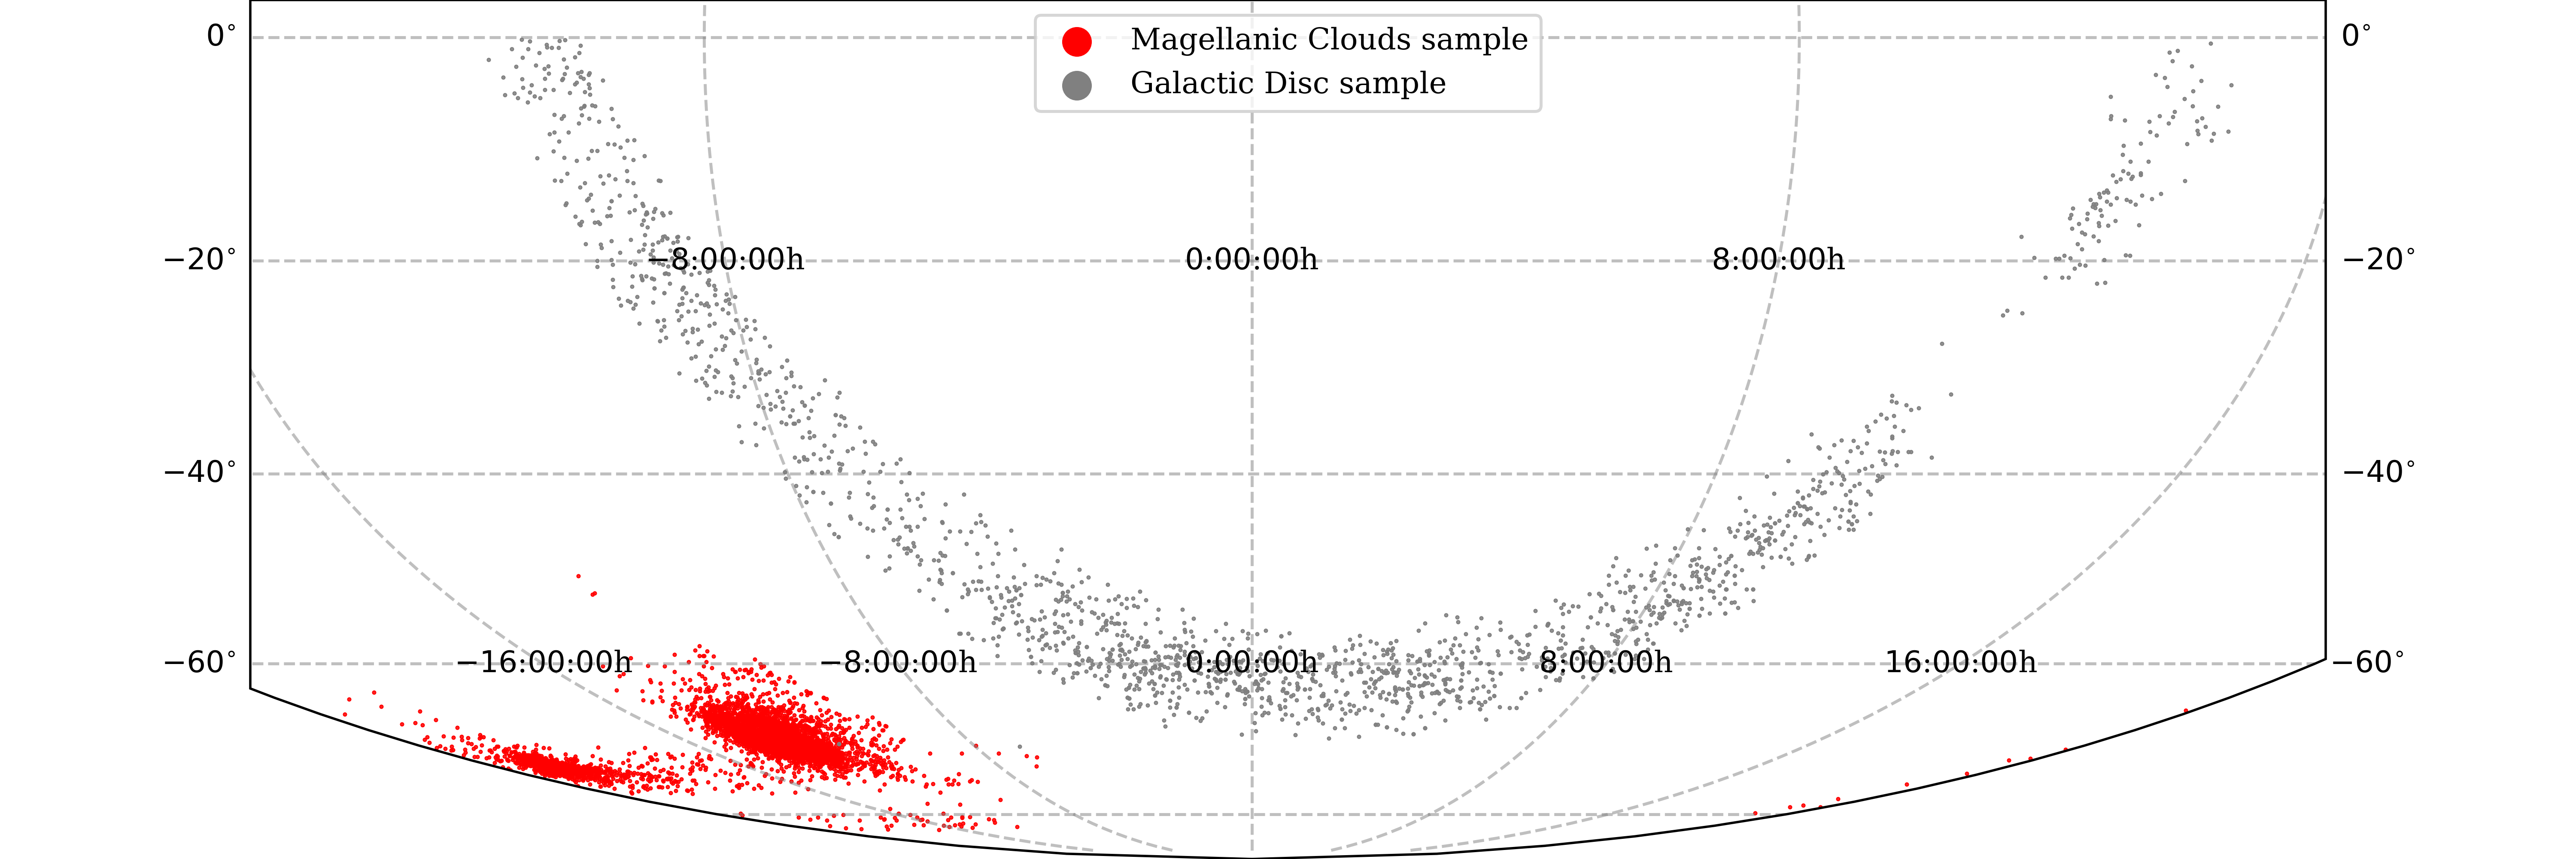
\includegraphics[scale=0.38]{plots/map_sample.png}
    \end{center}
    \caption{Distribution of objects in each sample.}
\end{figure}

Each object was analysed using ANOVA (analysis of variance) method \citep{schwarzenberg-czerny_advantage_1989} in order to determine period of light curve.
Then each light curve was fitted with four harmonic model
\begin{equation}\label{harm}
    I(t)=A_0+\sum_i^4 A_{1i}\sin{\left(2\pi i\frac{t}{P}\right)}+A_{2i}\cos{\left(2\pi i\frac{t}{P}\right)}
\end{equation}
with sigma clipping threshold set at $3\sigma$. Subsequently minimum mass ratio $q_{mmr}$ together with it's lower bound $\tilde{q}_{mmr}$ were calculated and previously described procedure was carried out.
In each sample objects with light curves indicating other type of variability then ellipsoidal one were removed together with those with period higher then
$50$ d. As we assume objects should be composed of star nearly filling Roche lobe suggesting rather small period. Exact value of threshold can be debated, here it's used as mean to 
remove pulsating stars that pollute our sample. After this part of preprocessing pipeline only $41$ objects from first sample left together with $22$ objects from second sample.
\section{Spectral Energy Distribution}
Each object was cross matched  with Gaia DR3 catalogue obtaining parallax (denoted from here as $\pi_0$ together with uncertainty denoted as $\sigma_{\pi}$) estimates of objects. If parallax was statistically significant ($\pi>3\sigma_{\pi}$)
it was used to derive distance to object. For objects towards Magellanic Clouds many entries lacked statistically significant parallax indicating that they really reside in Magellanic Clouds
and do not line up accidentally.
In this case distance estimate $d_0$ and distance uncertainty $\sigma_d$ were based on the work \citep{jacyszyn-dobrzeniecka_ogle-ing_2016} assuming that presented distribution 
of cepheid reflects underlying distribution of stars in sample.
In the case of LMC and SMC assumed distance estimates were  $d_{LMC}=49.93\pm1.79$ kpc and  $d_{SMC}=64.62\pm4.95$ kpc respectively. 

To further investigate nature of objects spectral energy distribution analysis was 
performed with two models: single star model and double star model. Main goal of this type of analysis is to use photometry from various parts of spectra to
reconstruct whole spectral characteristic and hence obtain parameters of our object temperature.
Single star model depends on three free parameters: logarithm of temperature $\log_{10}T$ (measured in kelvins), logarithm of luminosity $\log_{10} L$ (measured in $L_{\odot}$) while third 
parameter was either parallax (if there was measured one) or distance if it wasn't available. In the case of double star model there were two additional parameters describing 
second star $\log_{10} T_2$ and $\log_{10} L_2$. In the case of the first model star was assumed to be main sequence object (MS) with $\log{g}=4$. In double star model more massive star 
was assumed to have $\log{g_1}=4$ as in the first case while second object was assumed to be a giant with $\log{g_2}=2$. Objects with statistically significant parallax were assumed to have 
solar like metallicity ($Z=0.013$) as objects reside inside galactic disc while objects in Magellanic Clouds 
were assumed to have metallicity equal to $Z=0.010$ in the case of LMC/MBR and $Z=0.005$ in the case of SMC.
BaSeL library of stellar spectra \citep{lejeune_standard_1998} was used to find spectrum for any given $\log_{10}{T}$, $\log_{10} L$, $d$ 
by means of interpolation as implemented in python library
\texttt{pystellibs}\footnote{https://github.com/mfouesneau/pystellibs}.
Theoretically calculated stellar spectrum is then processed using \texttt{pyphot}\footnote{https://github.com/mfouesneau/pyphot} 
Python library yielding observed magnitude in required filter.

In order to find set of best fitting parameters Bayesian approach was adopted. Let's denote set of observed magnitudes as $\tilde{m}_i$, theoretically predicted
magnitudes as $m_i$ while errors of magnitudes as $\sigma_i$. Let's denote $\mathcal{U}(a,b)$ to be uniform distribution with support in form of interval $[a,b]$ and $\mathcal{N}(\mu,\sigma^2)$ as
normal distribution with mean $\mu$ and variance $\sigma_i^2$. In order to prepare Bayesian model one need to specify probability distributions that allow to evaluate likelihood of 
data. Each of the observed magnitudes $\tilde{m}_i$ is expected to be normally distributed with mean $m_i$ and variance $\sigma_i^2$ while prior distributions on each of the three parameters
is either uniform in case of $\log_{10} T$ and $\log_{10} L$ or normal in case of distance or parallax. Detailed model can be written as:
\begin{align}
    \log_{10}{T}\sim \mathcal{U}(3.31,4.6)\\
    \log_{10}{L} \sim \mathcal{U}(-3,5)\\
    d \sim \mathcal{N}(d_0,\sigma_d^2) \textrm{ or } \\
    \pi \sim \mathcal{N} (\pi,\sigma_{\pi}^2)\\
    \tilde{m}_i\sim \mathcal{N}(m_i(\log_{10} T, \log_{10} L, d ),\sigma_i^2) \textrm{ or }\\
    \tilde{m}_i\sim \mathcal{N}(m_i(\log_{10} T, \log_{10} L, \pi ),\sigma_i^2)
\end{align}
where  $m_i(\log_{10} T, \log_{10} L, d )$ is written to indicate that predicted magnitude is function of parameters. 
Similarly we can write down our second model together with priors for parameters
\begin{align}
    \log_{10}{T_1}\sim \mathcal{U}(3.31,4.6)\\
    \log_{10}{L_1} \sim \mathcal{U}(-3,5)\\
    \log_{10}{T_2}\sim \mathcal{U}(3.444,4.21)\\
    \log_{10}{L_2} \sim \mathcal{U}(-3,5)\\
    d \sim \mathcal{N}(d_0,\sigma_d^2) \textrm{ or } \\
    \pi \sim \mathcal{N} (\pi,\sigma_{\pi}^2)\\
    \tilde{m}_i\sim \mathcal{N}(m_i,\sigma_i^2)
\end{align}
where we hidden explicit dependence of $m_i$ on parameters for clarity. In both case we trancute our normal distribution to positive numbers as we do 
not permit negative parallax/distance. Range on the logarithm of temperature is limited due to boundaries of library while limit of the logarithm of luminosity is 
set in the boundaries in order to eliminate possible unphysical solutions.
Under those assumptions log-likelihood function can be written as 
\begin{align}
    \mathcal{L}=-\sum_i\frac{(\tilde{m}_i-m_i)^2}{2\sigma_i^2}-\frac{(d-d_0)^2}{2\sigma_d^2} \textrm{ or }\\
    \mathcal{L}=-\sum_i\frac{(\tilde{m}_i-m_i)^2}{2\sigma_i^2}-\frac{(\pi-\pi_0)^2}{2\sigma_{\pi}^2}
\end{align} depending whether distance or parallax was used. 

Following catalogues were used to assemble SEDs:
\begin{enumerate}
\item Catalogues shared by both samples of objects:
\begin{itemize}
    \item 2MASS survey \citep{skrutskie_two_2006}
    \item Gaia DR2 \citep{gaia_collaboration_gaia_2018}
    \item VISTA Hemisphere Survey DR5 \citep{mcmahon_vizier_2021}
    \item ALLWISE/WISE survey \citep{wright_wide-field_2010} \citep{cutri_vizier_2021}
    \item GALEX Survey \citep{bianchi_galex_2011}
    \item Spitzer IRAC data \citep{meixner_spitzer_2006}
    \item Denis survey  \citep{denis_vizier_2005}
    \item SkyMapper DR2 \citep{wolf_skymapper_2018} \citep{onken_skymapper_2019}
    \item XMM Optical Monitor data \citep{page_xmm-newton_2012}
\end{itemize}
\item Catalouges exclusive to the Magellanic Clouds:
\begin{itemize}
    \item VISTA Magellanic Cloud survey DR4 \citep{cioni_vizier_2017}
    \item Denis cataloug of objects in Magellanic Clouds \citep{cioni_denis_2000}
    \item Magellanic Clouds Photometric Survey: SMC and LMC \citep{zaritsky_magellanic_2002} \citep{zaritsky_magellanic_2004}
\end{itemize}
\item Catalouges exclusive to the Galactic Disc:
\begin{itemize}
    \item Bochium Galactic disc survey \citep{hackstein_bochum_2015}
    \item AAVSO Photometric All Sky Survey DR9 \citep{henden_apass_2015}
    \item VISTA Variable in Via Lactea Survey DR2 \citep{minniti_vizier_2017}
\end{itemize} 
\end{enumerate}. In the case of magellanic clouds extinction estimates were based on the map \citep{skowron_ogle-ing_2021} while in the case of Galactic disc extinction
was obtained using \texttt{mwdust} \citep{bovy_galactic_2016} Python library with 3D dust map beeing combination of \citep{green_3d_2019}, \citep{greiner_unusually_2001},
\citep{drimmel_three-dimensional_2003}. In the calculations Cardeli extinction law was assumed \citep{cardelli_relationship_1989}
and python implementation from \texttt{extinction}\footnote{https://extinction.readthedocs.io/en/latest/index.html} was used.
Using described setup MCMC python based library \texttt{emcee}\footnote{https://emcee.readthedocs.io/en/stable/} \citep{foreman-mackey_emcee_2013}
was used to construct compact library\footnote{https://github.com/Wesenheit/Iris} of routines used to sample from the posterior of our models allowing to estimates parameters together
with associated uncertainties. In order to help to decide between models 
BIC score was used 
\begin{equation}
    BIC=k\log{n}-2\mathcal{L}
\end{equation} where $k$ is number of estimated parameters and $n$ is  number of data points. Based on properties of SED $16$ final candidates were selected as objects with probable 
compact object companion. Complete list of objects together with key parameters is listed in table (ref).

\chapter{Results}
\section{}
\chapter{Summary}

\bibliography{Bachelor} 
\bibliographystyle{mnras}
\end{document}